\documentclass[../main.tex]{subfiles}

\begin{document}

\renewcommand{\labelitemi}{\ding{226}}
\renewcommand{\labelitemii}{\ding{227}}

\part{Heavy neutrino study}

\chapter{Prospects in T2K}


In the current work we study a possibility of the improvement of the constraints on the mixing elements of the HNL in the T2K experiment. The details about the experimental setup are described~in~the~\autoref{T2K:general}. The main feature of the experiment for the HNL search is very intensive proton beam providing by J-PARC accelerator. The beam operation is overviewed~in~the~\autoref{T2K:nu_beam}. The focusing system allow to perform the analysis focusing positive or negative mesons from the proton interactions. As mentioned in the \nameref{intro:HNL}, heavy neutrinos could be produced in the mesons decays. As a result there are two possible strategies of the HNL search:
\begin{itemize}
    \item measurement of the meson decay kinematics. The effect is proportional to $\left|U_l\right|^2$;
    \item search for decay products of the heavy neutrino. As both HNL production and decay are proportional to $\left|U_l\right|^2$, the final effect $\propto\left|U_l\right|^4$.
\end{itemize}

The schema of the T2K experiment is shown in~\autoref{fig:HNL:t2k_schema}. The muon monitor is the only instrument that could measure the muons directly from the meson decay. In spite of its extreme usefulness for the neutrino beam intensity and direction measurements, it could not provide necessary precision for the search of the HNL through the detection of the muons from the meson decay. Thus the only way of the heavy neutrino study in the T2K is search for the HNL decays in the near detector complex. The near detector complex (\autoref{T2K:nd}) consists of on-axis INGRID detector and off-axis ND280. The most precise analysis could be done with the the ND280's time projections chambers. As we are looking for the HNL decays in the neutrino beam the gaseous detectors will observe much less background from the neutrino interactions comparing to scintillators.

\begin{figure}[h!]
    \centering
    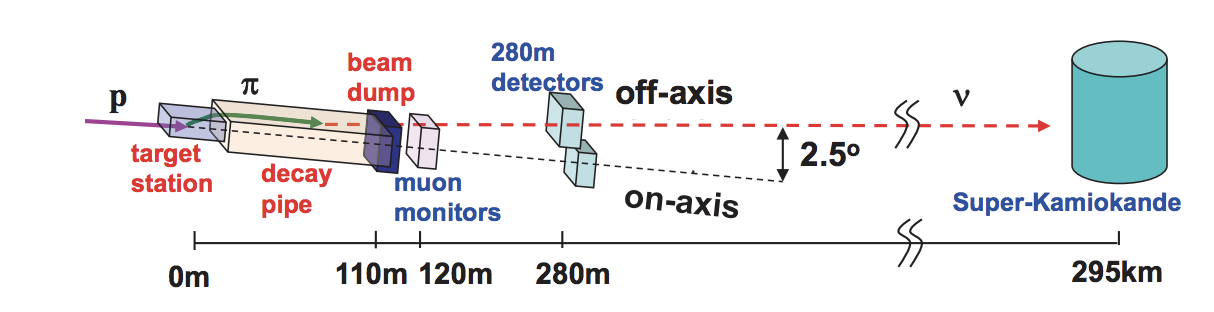
\includegraphics[width=\linewidth]{t2k_schema.png}
    \caption{A schematic view of the neutrino beamline and the detectors in the T2K experiment.}
    \label{fig:HNL:t2k_schema}
\end{figure}

With the 30 $GeV/c$ proton beam mainly pions are produced with some fractions of kaons. The comparison of the neutrino flux from different parent particles are presented~in~\autoref{fig:HNL:meson_flux}. As we want to study the maximum range of the HNL mass we will concentrate on the kaon decays. Thus we will be able to study the mass region up to 493 $MeV/c^2$. The overview of the HNL nature including the relation with the Standard Model particles is presented~in~\autoref{intro:HNL}. The particular production and decay modes of the heavy neutrino masses that are available for the analysis in our experiment are summarized in the kinematic scheme in~\autoref{fig:HNL:mass_scale} with specific HNL mass region for each of them.

\begin{figure}[h!]
    \centering
    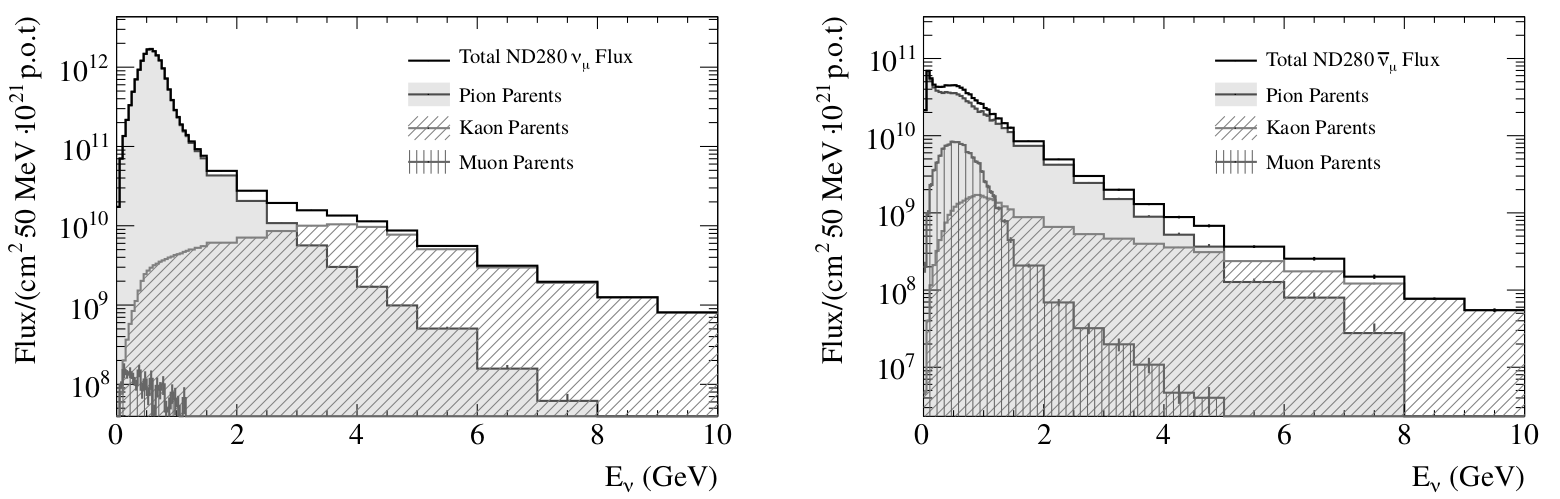
\includegraphics[width=\linewidth]{meson_flux}
    \caption{The muon neutrino and anti-neutrino flux prediction at the ND280 broken down by the neutrino parent particle type.}
    \label{fig:HNL:meson_flux}
\end{figure}

\begin{figure}[h!]
    \centering
    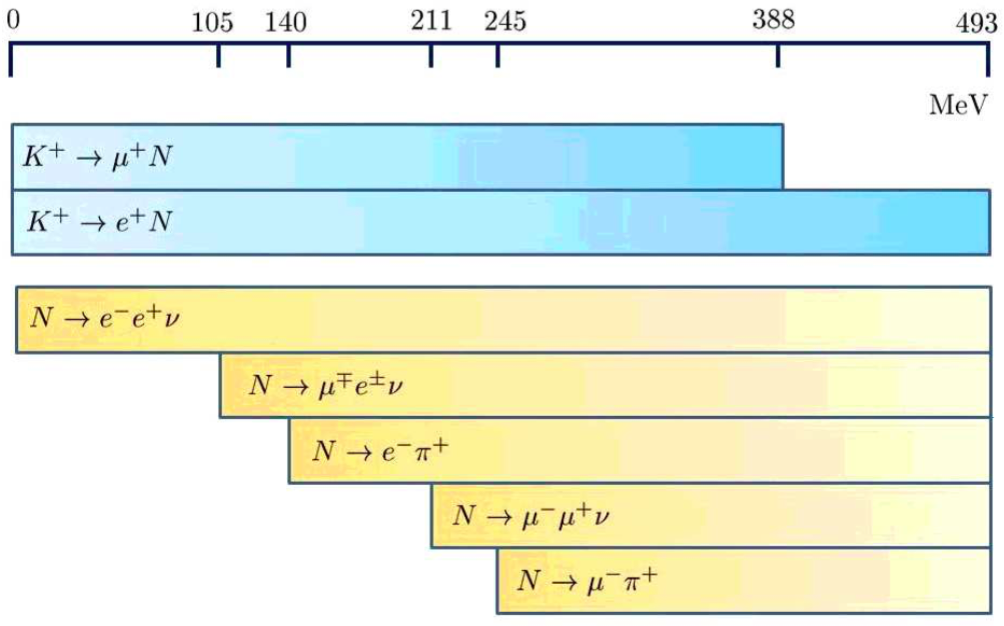
\includegraphics[width=0.7\linewidth]{HNL_mass_scale}
    \caption{Summary of the production and detection processes of the heavy neutrino available for the analysis with the ND280. The horizontal axis corresponds to the HNL mass}
    \label{fig:HNL:mass_scale}
\end{figure}

As one can see from the scheme in our study we will concentrate on the two and tree body decays of the heavy neutrino.

\begin{eqnarray}
    &N\to\ell^{\pm}\pi^{\mp} &\\
    &N\to\ell^{\pm}\ell^{\mp}\nu & \\
\end{eqnarray}

We would like to highlight the importance of the study of a HNL dimuon decay mode: $N\to\mu\mu\nu$. This decay has charge and neutral current contributions shown in Fig.~\ref{fig:DimuonFeynman} (from~\cite{Johnson1997}).

\begin{figure}[h!]
    \begin{minipage}[h]{0.49\linewidth}
        \center{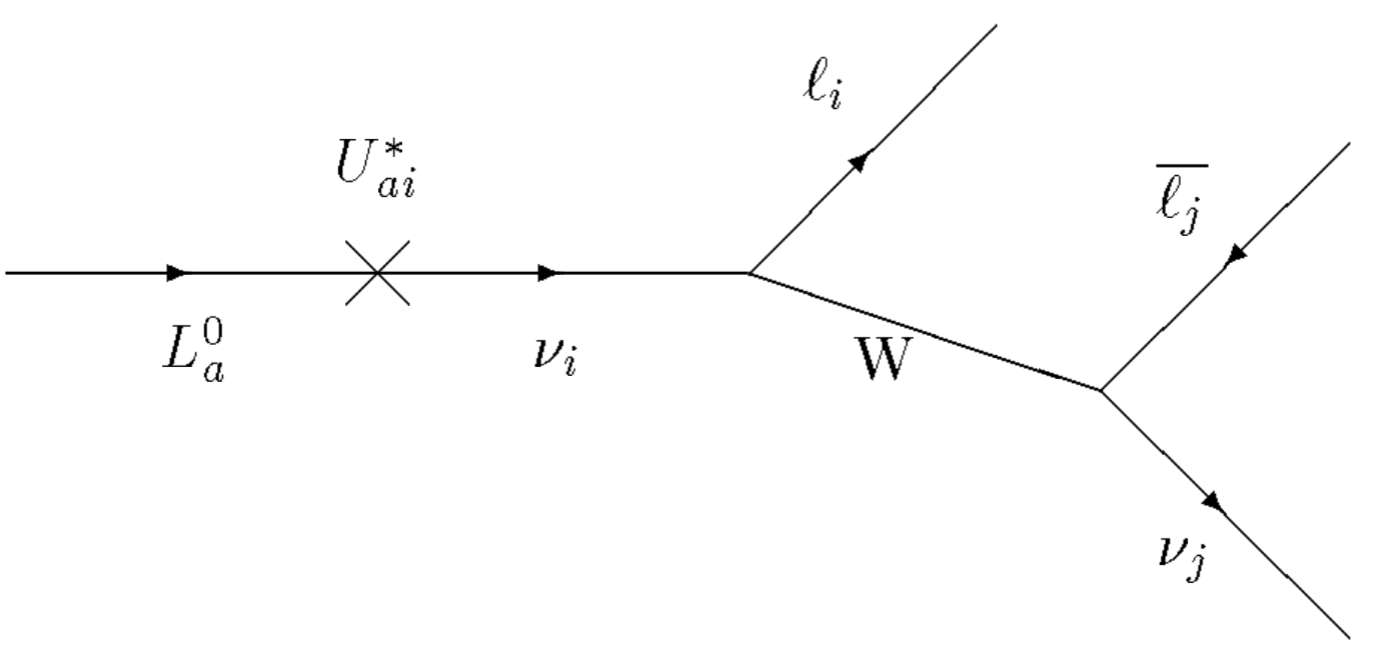
\includegraphics[width=\linewidth]{DiMuonCC.png} \\ a) }
    \end{minipage}
    \hfill
    \begin{minipage}[h]{0.49\linewidth}
        \center{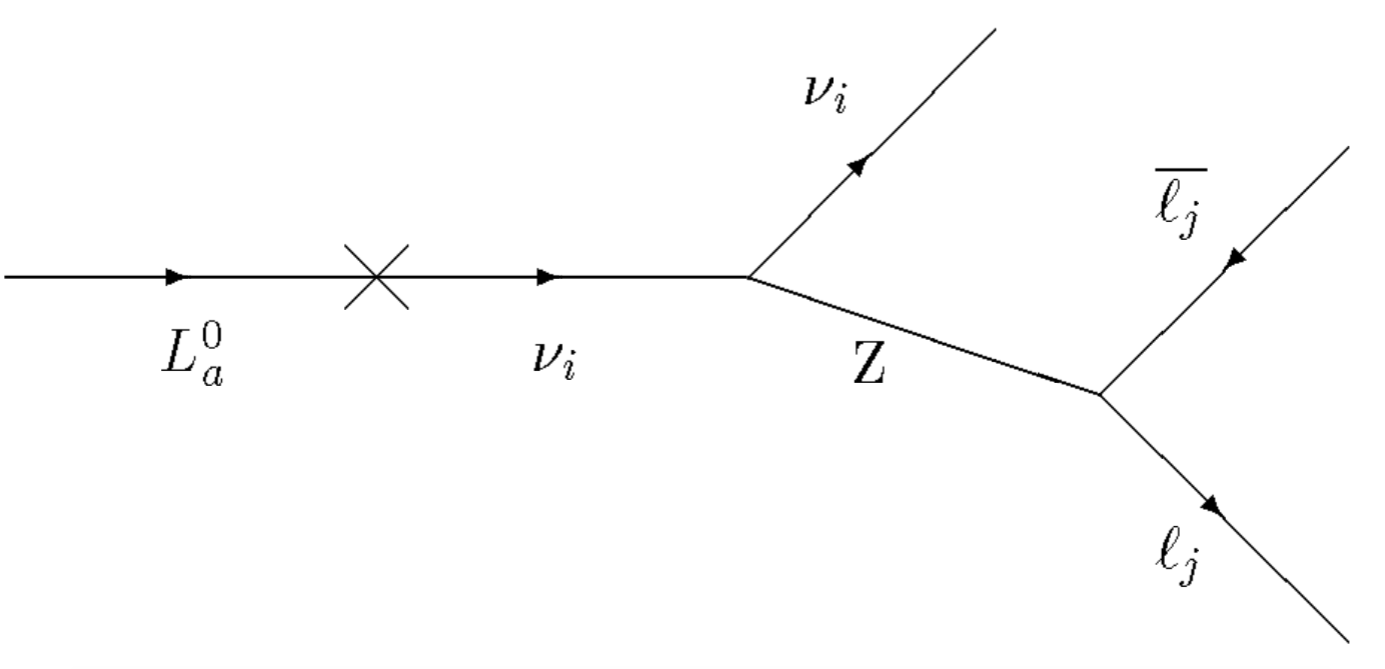
\includegraphics[width=\linewidth]{DiMuonNC.png} \\ b)}
    \end{minipage}
    \caption{Feynman diagrams for the HNL decay $N\to\mu\mu\nu$ via charged (a) and neutral (b) current.}
    \label{fig:DimuonFeynman}
\end{figure}

If the HNL decays via NC, any type of the active neutrino could be produced ($\nu_{e}, \nu_{\mu}, \nu_{\tau}$), so we can study the mixing element including $|U\tau|$. This is interesting as the upper limits on this element are rather high\todo{reference to the figure in intro}.

The first one requires applying some simple cuts and then study difference between data and MC estimation with a peak shape. We need a rather accurate background prediction for this method. Also invariant mass resolution is one of the most important issue. We have studied the possible resolution for the HNL signal samples. The events that pass all the cuts described in the~\autoref{HNL:sel} give as the reconstructed mass distribution. The examples of such distribution are presented in~\autoref{fig:HNL:InvMass}. The resolution of the invariant mass reconstruction on the HNL mass is shown in~\autoref{fig:HNL:InvMassPlot}. As one can see, RMS is quite large $\approx70MeV$. The main background processes for the HNL decay are  interactions of the active neutrinos. In near detector there are three TPCs filled with argon gas. The cross sections of the neutrino interactions in gas are not studied well. Studies of these events were performed by ArgoNeuT group~\cite{Acciarri2014}. In our momentum region ($\approx1GeV$) the uncertainties are relatively large. Other background processes can be $K^0, \Lambda, \eta$ decays, deep inelastic neutrino scattering, etc. (\autoref{HNL:bg}) that are also poorly studied. Because of this we can not provide needed accuracy of the background prediction and the method of the invariant mass peak search can not be applied.
\begin{figure}[h!]
    \begin{minipage}[h]{0.49\linewidth}
        \center{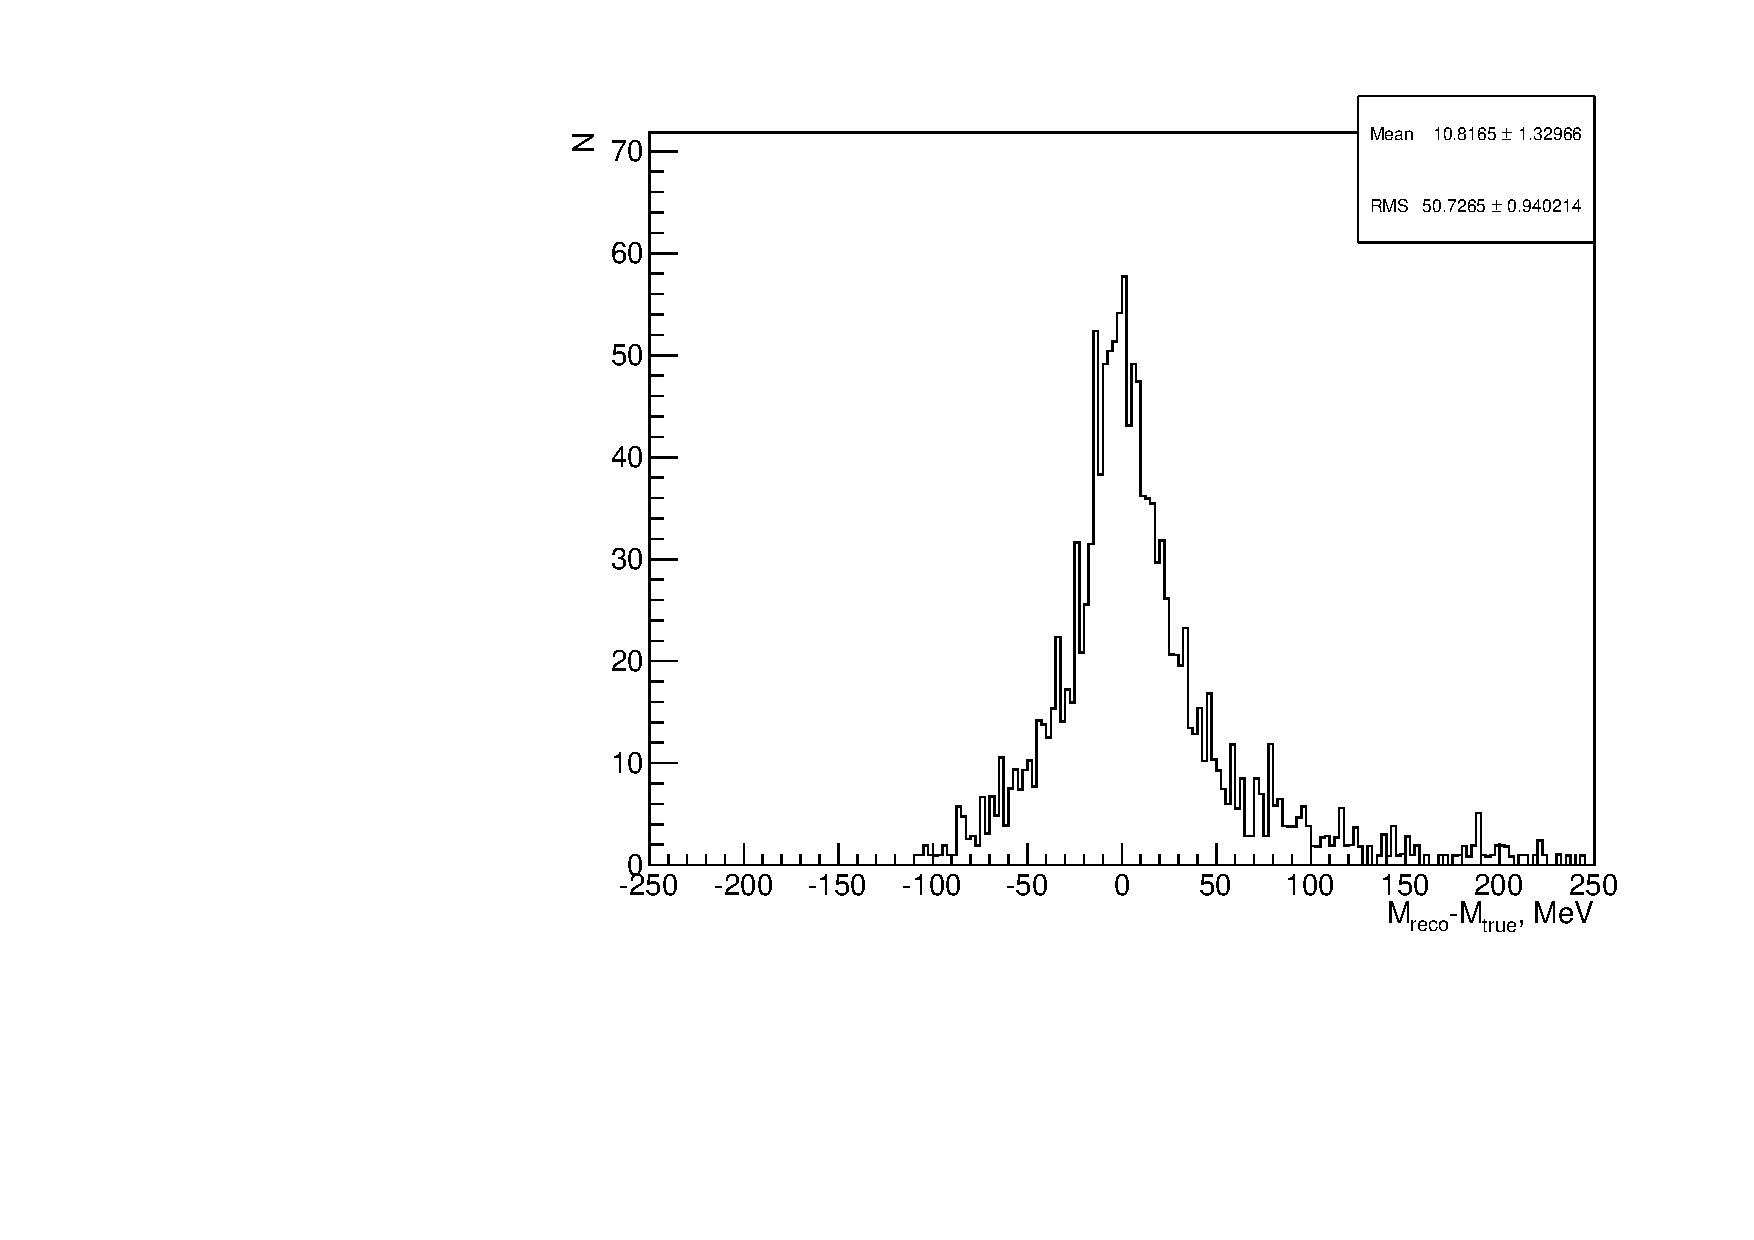
\includegraphics[width=\linewidth]{InvMass036}}
    \end{minipage}
    \hfill
    \begin{minipage}[h]{0.49\linewidth}
        \center{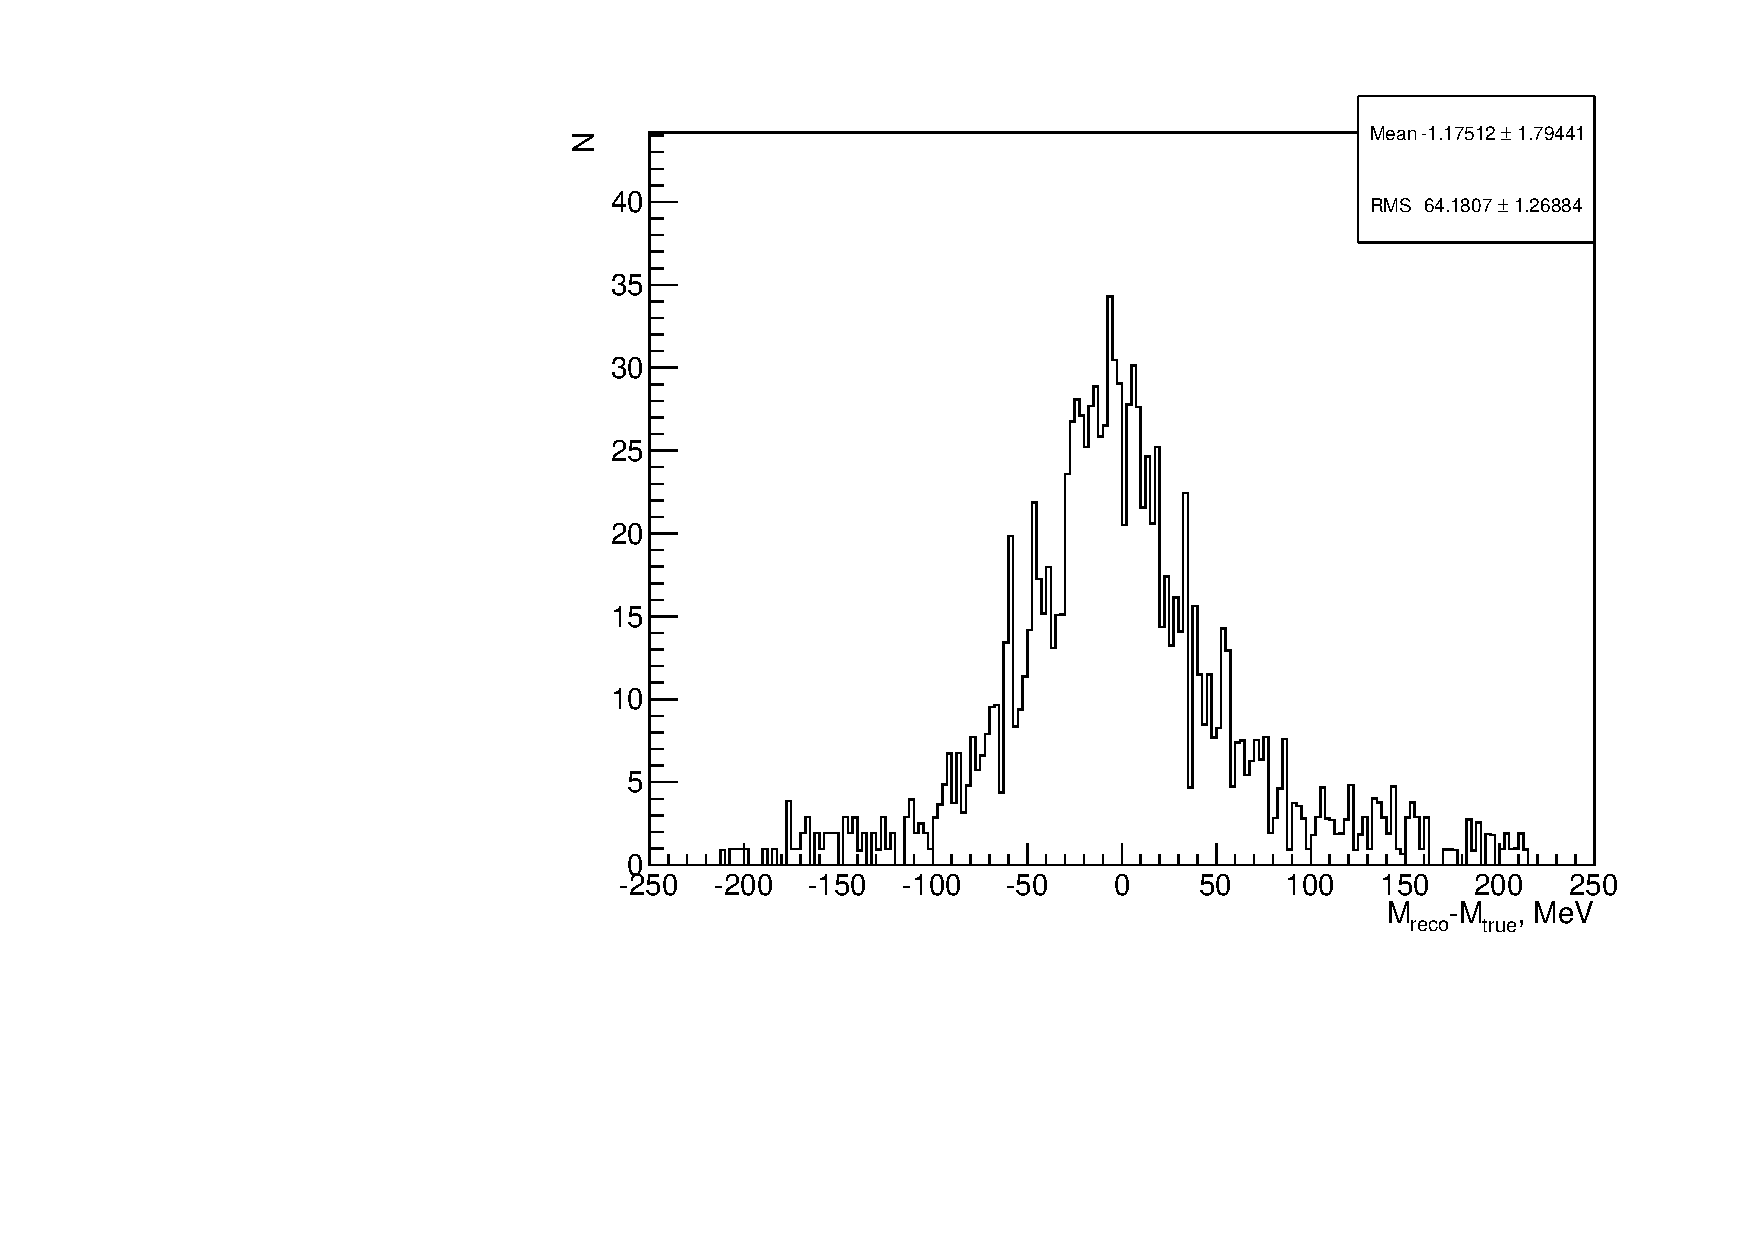
\includegraphics[width=\linewidth]{InvMass048}}
    \end{minipage}
    \caption{HNL invariant mass resolution. Left is for $M_{HNL}=360$ MeV, right is for $M_{HNL}=480$ MeV for the $\mu\pi$ mode.}
    \label{fig:HNL:InvMass}
\end{figure}

\begin{figure}[h!]
    \begin{minipage}[h]{0.49\linewidth}
        \center{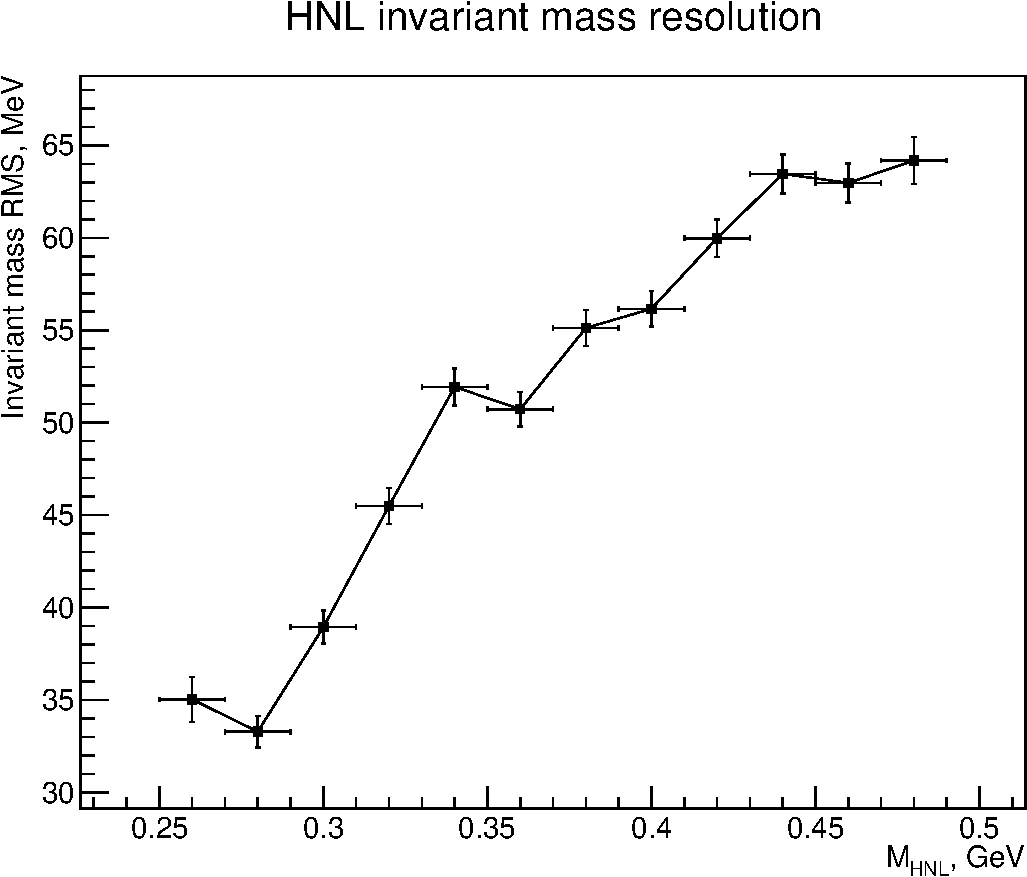
\includegraphics[width=\linewidth]{InvMassMuPlot} \\ a)}
    \end{minipage}
    \hfill
    \begin{minipage}[h]{0.49\linewidth}
        \center{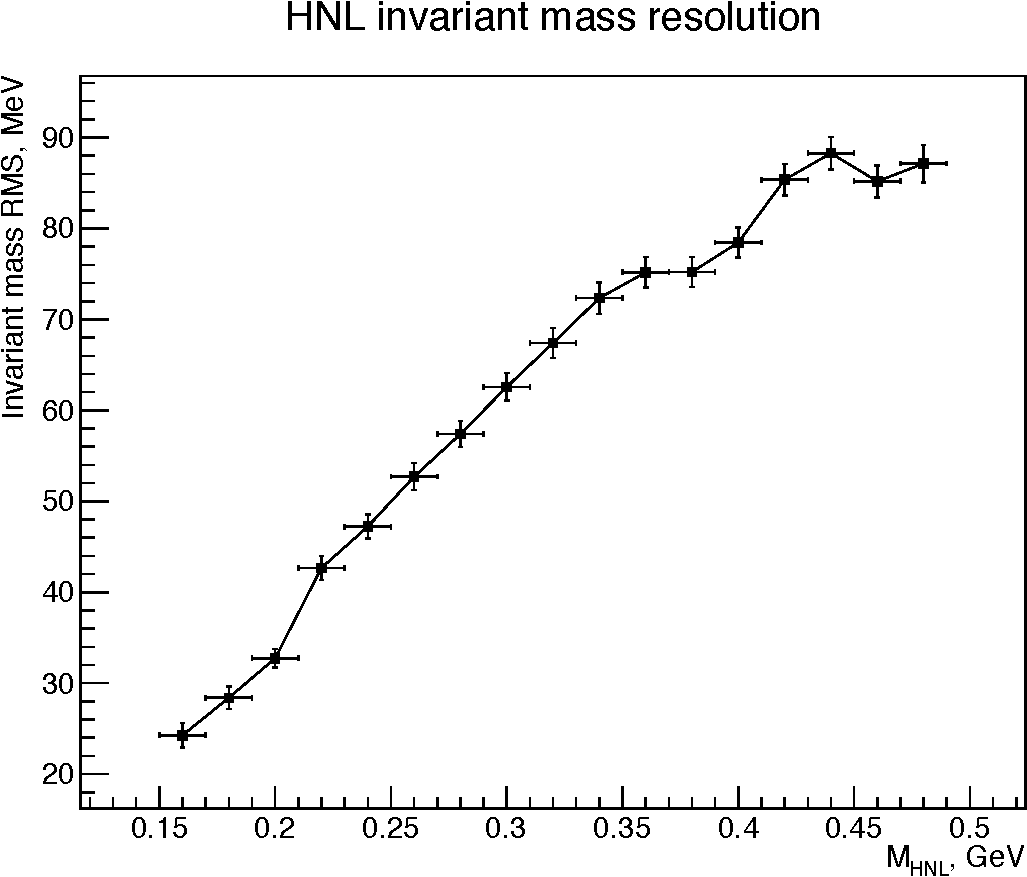
\includegraphics[width=\linewidth]{InvMassElePlot} \\ b) }
    \end{minipage}
    \caption{HNL invariant mass resolution (RMS) dependence on the HNL mass for (a) $N\to \mu\pi$ mode and (b) $N\to e\pi$ mode.}
    \label{fig:HNL:InvMassPlot}
\end{figure}








\begin{comment}

The T2K experiment uses neutrino beam from $\pi^\pm$ and $K^\pm$ decays. In our study a search of HNL from both $K^+$ and $K^-$ decays is carried out in order to increase sensitivity because of the larger statistics. We assume the Majorana nature of a HNL, this allows to study decays of $K^+$, $K^-$ and both decay modes of a heavy neutrino to $\ell^{\pm}\pi^{\mp}$.

As we focus on search of the HNL decay there are two analysis methods:
\begin{itemize}
  \item search for a peak in the HNL candidate invariant mass spectrum
  \item search for a rare event in a low background environment
\end{itemize}

The first one requires applying some simple cuts and then study difference between data and MC estimation with a peak shape. We need a rather accurate background prediction for this method. Also invariant mass resolution is one of the most important issue. We have studied the possible resolution for the HNL signal samples. The events that pass all the cuts described in the section~\ref{sec:Ana} give as the reconstructed mass distribution. The examples of such distribution are presented in Fig.~\ref{fig:InvMass}. The resolution of the invariant mass reconstruction on the HNL mass is shown in Fig.~\ref{fig:InvMassPlot}. As one can see, RMS is quite large $\approx70MeV$. The main background processes for the HNL decay are  interactions of the active neutrinos. In near detector there are three TPCs filled with argon gas. The cross sections of the neutrino interactions in gas are not studied well. Studies of these events were performed by ArgoNeuT group~\cite{acciarri2014measurements}. In our momentum region ($\approx1GeV$) the uncertainties are really large. Other background processes can be $K^0, \Lambda, \eta$ decays, deep inelastic neutrino scattering, etc. (Sec~\ref{sec:bg}) that are also poorly studied. Because of this we can not provide needed accuracy of the background prediction and the method of the invariant mass peak search can not be applied.
\begin{figure}[H]
    \begin{minipage}[h]{0.49\linewidth}
        \center{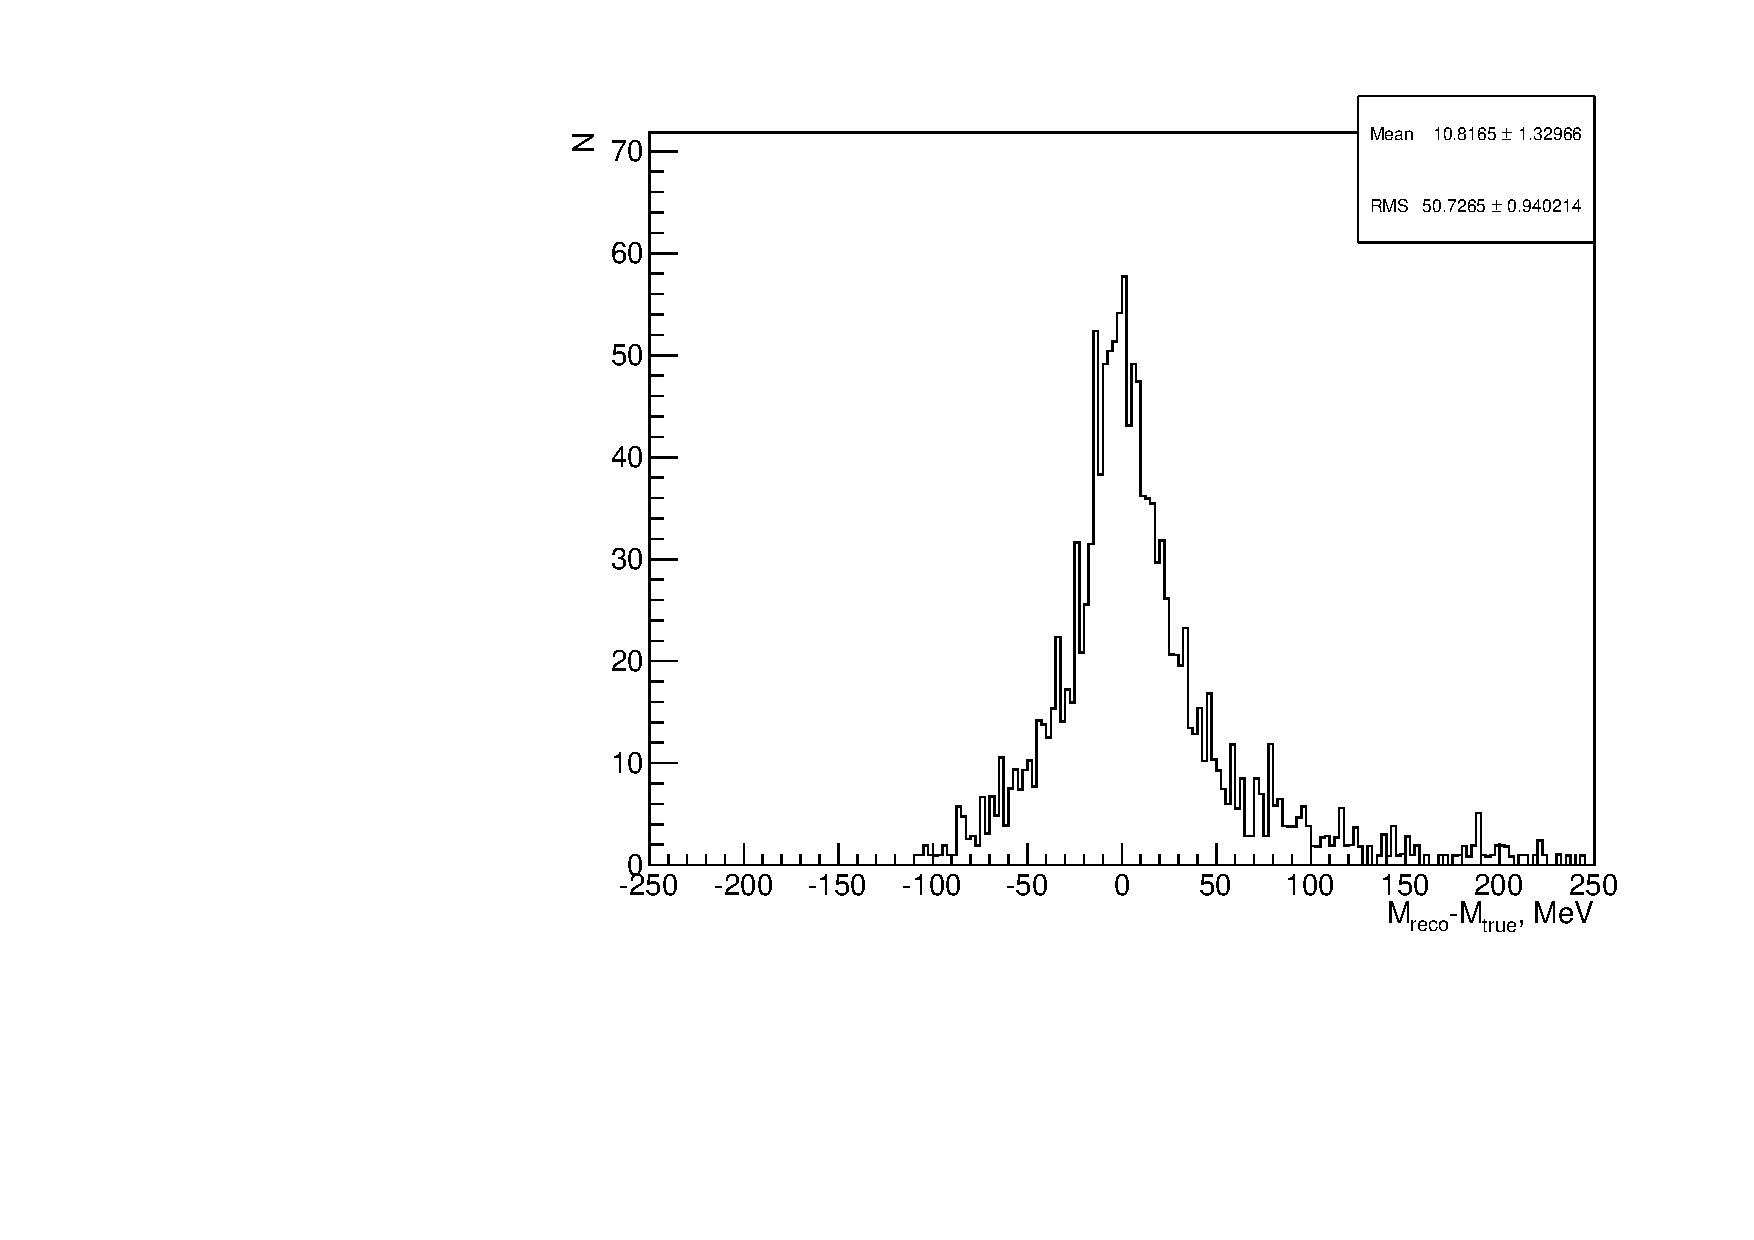
\includegraphics[width=\linewidth]{InvMass036}}
    \end{minipage}
    \hfill
    \begin{minipage}[h]{0.49\linewidth}
        \center{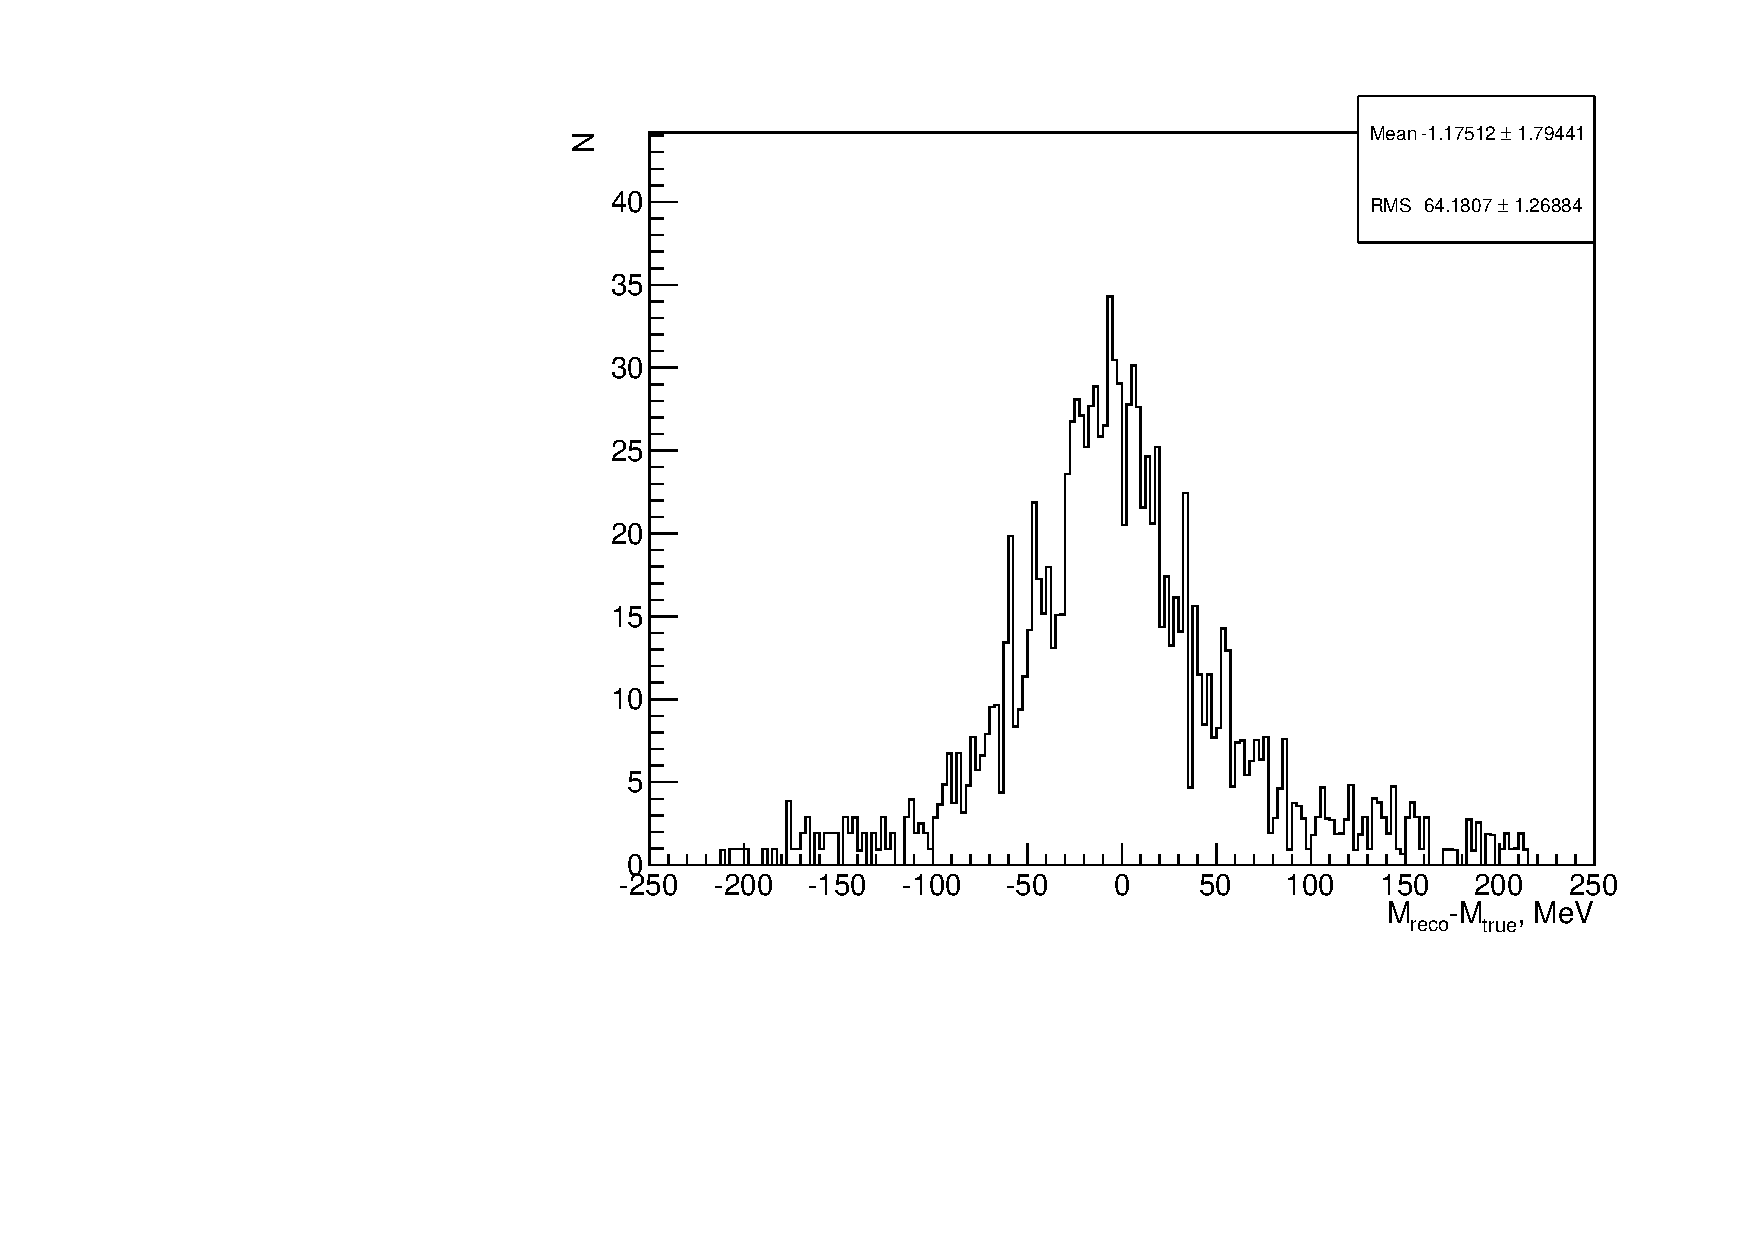
\includegraphics[width=\linewidth]{InvMass048}}
    \end{minipage}
    \caption{HNL invariant mass resolution. Left is for $M_{HNL}=360$ MeV, right is for $M_{HNL}=480$ MeV for the $\mu\pi$ mode.}
    \label{fig:InvMass}
\end{figure}

\begin{figure}[H]
    \begin{minipage}[h]{0.49\linewidth}
        \center{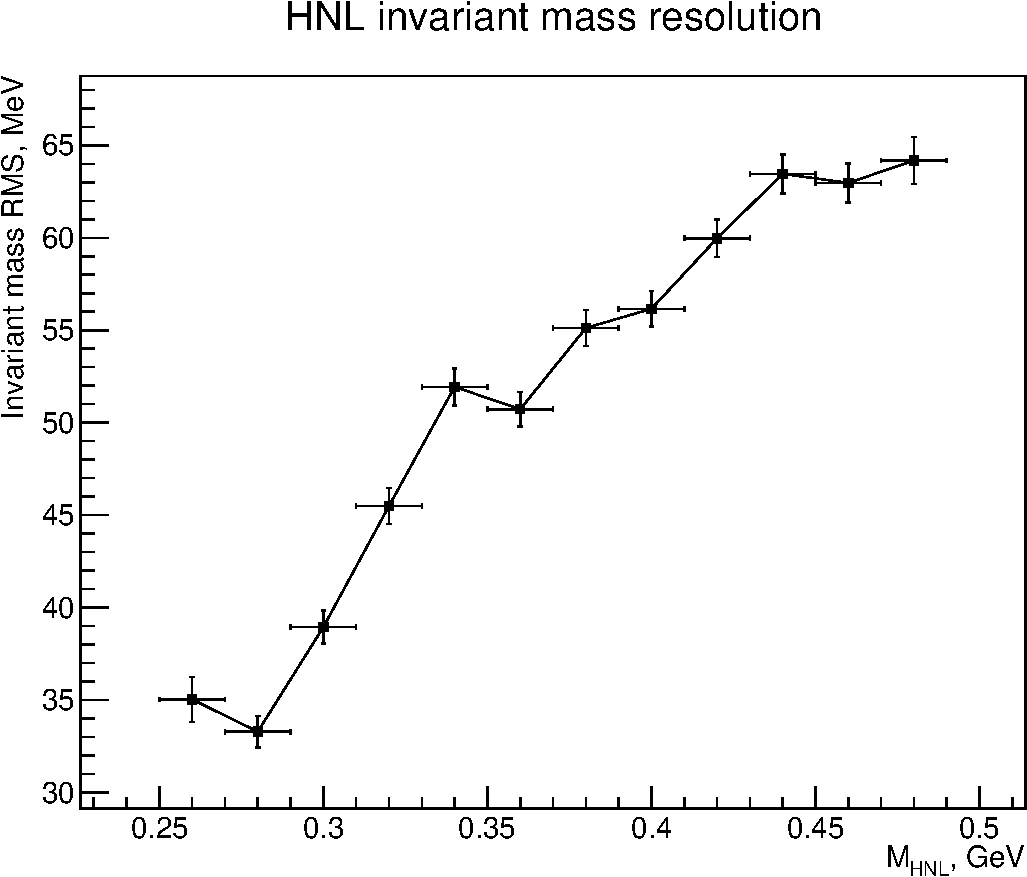
\includegraphics[width=\linewidth]{InvMassMuPlot} \\ a)}
    \end{minipage}
    \hfill
    \begin{minipage}[h]{0.49\linewidth}
        \center{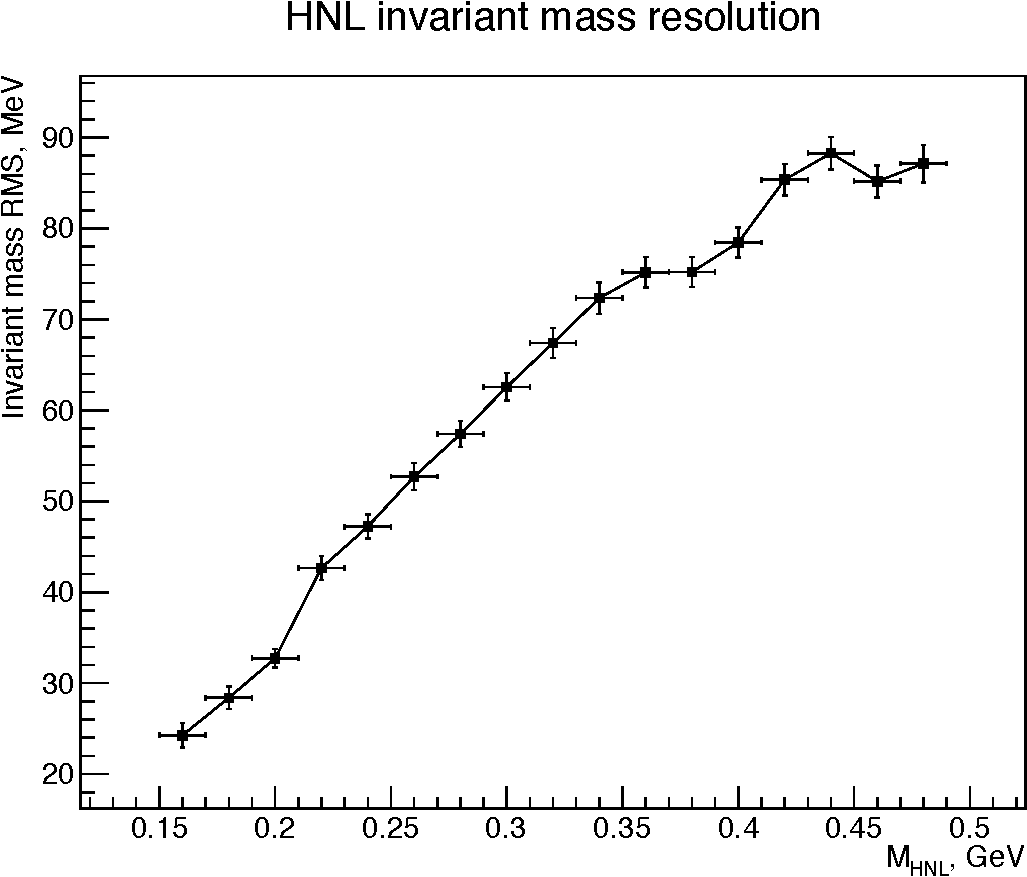
\includegraphics[width=\linewidth]{InvMassElePlot} \\ b) }
    \end{minipage}
    \caption{HNL invariant mass resolution (RMS) dependence on the HNL mass for (a) $N\to \mu\pi$ mode and (b) $N\to e\pi$ mode.}
    \label{fig:InvMassPlot}
\end{figure}

The second method requires the cut sequence for the background elimination. Then we can use low signal statistical approach which is described in Sec.~\ref{sec:LowSignal}. For background suppression we decided to use only fiducial volume of the TPCs. The difference of the density between the gas (TPC) and the scintillator (FGD) is large. As number of the active neutrino interactions depends on density, this method provides significant background reduction.

As described, the cross-section uncertainties of the active neutrino interactions in gas are large. Because of this, we are going to treat all the events that survive after all cuts applied as signal and put the constraints on mixing elements. The details of this approach is described in the next section.

\subsection{Low level signal analysis}
\label{sec:LowSignal}

The statistical approach to the low level signal analysis is described in the Highland and Cousins work~\cite{cousins1992incorporating}. As number of the HNL decay events is proportional to the forth power of the mixing element, constraints on $\left|U_i\right|^2$ without systematics looks like:
\begin{equation}
  \left|U_i\right|^2_{limit}=\sqrt{\frac{U_n}{N_{events}}}
  \label{eq:constraints}
\end{equation}
where $i=e,\mu$, $U_n$ is 90\% C.L. Poisson limit for $n$ observed events and $N_{events}$ is expected number of signal events assuming $\left|U\right|^2=1$. If we take into account the detector acceptance uncertainty, the result can be calculated according to Ref.~\cite{cousins1992incorporating}:
\begin{equation}
  U_n=U_{n0}\left\{1+E_n\frac{\sigma^2_{Acc}}{2}\left(1+\left(\frac{E_n\sigma_{Acc}}{2}\right)^2\right)\right\}
  \label{eq:constrainsAcc}
\end{equation}
where $U_{n0}$ is 90\% C.L. Poisson limit for $n$ observed events, $\sigma_{Acc}$ is the acceptance error, $E_n=U_{n0}-n$ represents the excess of the upper limit of
a Poisson parameter over the number n of observed events, for a specified confidence level. This approach can be applied only while $\sigma_{Acc}<1/E_n$. We will show that in our study $\sigma_{Acc}\approx0.3$ and $1/E_n>0.5$ (this values are described in the section~\ref{sec:syst}). So this method can be applied for the analysis.
\end{comment}




\chapter{HNL flux simulations}
\section{T2K flux simulation}
\section{HNL production}
\section{HNL decays}
\chapter{Analysis}
\label{HNL:ana}
\section{Event selection}
\label{HNL:sel}
\subsection{Signal event selection}
\subsection{Background suppression}
\label{HNL:bg}
\section{Systematic uncertainties}
\subsection{Detector systematics}
\subsection{Flux systematics}
\subsection{Pile up}
\section{Statistical methods}
\chapter{Results}
\section{MC sensitivity estimations}
\section{Data unbinding}
\end{document}